\documentclass[12pt]{article}
\usepackage[letterpaper, margin=1in]{geometry}
\usepackage{graphicx, subfigure, float}
\usepackage{placeins}
\usepackage{longtable}
\usepackage{multicol}
\usepackage{supertabular}
\usepackage{amsmath}
\usepackage{mathtools}
\usepackage{fancyhdr}
\usepackage{graphicx,rotating,booktabs}
\usepackage{blindtext}
\usepackage{array}
\usepackage[]{setspace}
\usepackage[backend=biber, style=apa]{biblatex}
\usepackage{titling}
\usepackage[pdftex]{hyperref}
\doublespacing

\PassOptionsToPackage{hyphens}{url}\usepackage{hyperref}


\pagestyle{fancy}
\fancyhf{}
\fancyhead[LE,RO]{}
\fancyhead[RE,LO]{}
\fancyfoot[RE,RO]{Hasler \thepage}

\renewcommand{\headrulewidth}{2pt}
\renewcommand{\footrulewidth}{1pt}

\newcolumntype{C}[1]{>{\centering\let\newline\\\arraybackslash\hspace{0pt}}m{#1}}

\begin{document}
	\begin{titlingpage}
	
	\title{The Gamble of ICT Infrastructure: A Formal Model of How Governments Build New Infrastructure}
	\author{Jack Hasler}
	\maketitle


	\begin{abstract}
	Numerous pieces of literature have come to the counterintuitive finding that advancing information and communications technologies (ICTs) can help a government monitor and control their population while also assisting the opposition in mobilizing and challenging that same government. Many others have used ICTs as independent variables to explain violence, protests, and public opinion. In this paper, I present a formal model that shows the risk of ignoring how these infrastructures are put in place. I argue that infrastructure projects are usually carried out regionally and not nationally, which allows governments to be selective about which rural areas they improve. This choice allows them to single out those that are friendly while ignoring those that would organize against them. 
	\end{abstract}

	\end{titlingpage}
	
	\section{Introduction}
	Information and communication technologies (ICTs) have spread to every country on the planet, but even the most common of them have yet to fully expand to every region or village within those countries. These technologies may be high-speed Internet, telephone (both cellular and mobile), television or radio, but they all serve a similar purpose of connecting people to other peoples and information they would not regularly come into contact with. They can also serve the important function of strengthening relationships between locals and making it easier for people in the same vicinity to quickly organize meetings.
	
	That the diffusion of these technologies varies should not come as a surprise. Across nations the differences are stark In 2016, only 7 cellular phones were in use in Eritrea per 100 people. Meanwhile, in the United Arab Emirates, that number was 204, meaning that the average person had at least two personal phones (World Bank 2016). Within them, too, the level and type of technological diffusion differs considerably. One need only consult the AT\&T coverage map in Figure 1 to see that even though the U.S. has considerable mobile phone coverage in 2017, there are still many areas that lack adequate connections. Broadband Internet, a service that is as important if not more so for some than phone access, lacks even 10\% coverage in some parts of the United States. Many that live in rural locations cannot access Internet at home without connecting to a satellite, a tedious process that takes at least ten seconds to load a single web page. Figure 2 shows in the late 2000s the availability of 4 mbps internet across the United States, but a recent NPR report highlighted the continued problems surrounding access to Internet in the rural areas of Pennsylvania (NPR 2017). According to World Bank statistics, only 32 out of 100 people in the United States have a broadband Internet subscription, placing them 27th in the world. For some countries like Nigeria and Haiti, however, that number is about .01 people (World Bank 2016).
	
	\begin{figure}[H]
		\centering
		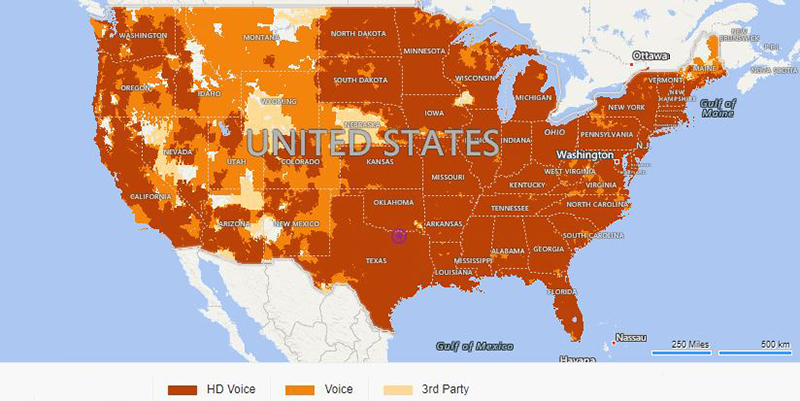
\includegraphics[width=0.7\linewidth]{at&t-coverage-map}
		\caption{AT\&T Coverage 2017 Source: https://www.att.com/maps/wireless-coverage.html}
		\label{fig:att-coverage-map}
	\end{figure}
	\begin{figure}[H]
		\centering
		\includegraphics[width=0.7\linewidth]{"us broadband"}
		\caption{U.S. Broadband Coverage in 2009 Source: http://www.broadband.gov/plan/3-current-state-of-the-ecosystem/}
		\label{fig:us-broadband}
	\end{figure}
	
	This variation in ICT has been used by a number of scholars, both within and between nations to help explain intrastate conflict, protests, and democratization among other topics. These works often gloss over, however, important endogeneity issues related to how those technologies were introduced to begin with. In any location where businesses do not see a profit in providing one of these services, the local, regional, or national government must decide whether to subsidize it, provide it themselves, or allow the area to go without. Since much of the literature that uses these metrics at least implicitly involves a government, understanding when and why an ICT infrastructure is introduced is critical to understanding and critiquing the research.
	
	This paper proceeds in three parts. First, I characterize the literature to date, careful to note who does and does not address this important issue. Second, I suggest a relatively simple model of government decision making. Third and finally, I provide of sketch of the case study I am currently gathering data for and lay out future extensions for work involving formal models on this subject as well as provide empirical suggestions for future research.
	
	\section{The Uses of ICT as a Independent Variable}
	In the last decade, new research linking ICTs, especially social media and cell phones, has taken on the older question of what causes democratization. Two contradicting theories linking technology and democracy have been advanced. First, greater amounts of information may lead to democratization as ideas circulate more widely encouraging protests and other types of dissent while lessening the autocrat’s control of the people (e.g. Reuter and Szakonyi 2015; Diamond 2010). Second, a freer flow of information may help the autocrat maintain control by providing them with an easier means to monitor dissent and locate individuals or groups that can pose a challenge (e.g. Egorov, Guriev, and Sonin 2009; King, Pan, and Roberts 2013; Rød and Weidmann 2015). Most of this literature acknowledges that the creation of an ICT infrastructure (whether for cell phones or Internet) is an endogeneity concern, but they rarely consider it below the national level. 
	
	To complicate matters further, cases, such as China, exist that appear to illustrate both democratization dynamics, which leaves open the question of whether technology has different effects conditional on some other independent variable or if one or both arguments are simply wrong. The model in this paper does not attempt to adjudicate between these literatures, but it does show that the endogeneity concern should be taken seriously not just at the national level, but at the subnational levels as well. It has the added benefit of applying to all governments, which allows a discussion about democratization processes inside of countries that may be nominally or even mostly democratic. In other words, while most of the existing works focus on the negative half of the Polity scale, my model works well in the positive half as well.
	
	Other scholars have connected ICT use to civil wars (Dixon 2009, Kalyvas and Balcells 2010), corruption (Bailard 2009), protests more generally (Crabtree et al. 2015; Hussein and Howard 2013; Little 2015) and polling in the United States (Bimber 2001; Keeter 2006). While these dependent variables have little in common, the mechanisms proposed tend to mirror those discussed above. Either individuals and groups in power use the new ICTs to monitor and control or their opponents use them to overcome Olsonian coordination issues. 
	
	Although many scholars have studied ICTs, they have tackled it using different empiric metrics. Internet subscriptions, telephone usage (both fixed and cellular), and energy consumption have all been used. As Kramon and Posner (2013) warn about measuring the benefits of distributive politics, the use of different proxies might noticeably impact the results. This is especially true for communication technologies because some forms may make others obsolete or unnecessary. For example, many areas of Africa never adopted fixed telephone lines because by the time they were able to build the infrastructure, cellular telephones were a better option. Likewise, the quantity and cost of international telephone calls is likely to be impacted by the amount of Internet service, which will allow individuals to fulfill the same need for no additional cost.
	
	In a recent review essay, Lyall and Dafoe (2015) identified numerous other methodological problems with the metric of mobile cellular subscriptions, which is the most often used proxy (e.g. Pierskalla and Hollenbach 2013; Shapiro and Weidmann 2015). Specifically, they argue that the metric is biased because more cellphones mean that it will also be easier to report episodes of violence. In fact, other scholars (Van der Windt and Humpreys 2016) have proposed distributing mobile phones in such areas for exactly this reason. Lyall and Dafoe also note that multiple studies hypothesize different causal pathways that cellular subscriptions might be linked to conflict, but none are explicitly tested. Similar problems plague most metrics of technological spread and are not limited to this specific independent variable. In fact, the role of railroad construction in the offense-defense balance has been debated for decades in the military effectiveness literature for similar reasons (Lieber 2000). 
	
	\section{A Model of ICT Extension}
	The model presented here is a fairly straightforward signaling model that takes advantage of the fact that an ICT infrastructure presents the potential for monetary gains to both the local people and the government but has the added risk to the government that they are not positive of the loyalty of the individuals in the area in question. The government would like to distribute new infrastructures exclusively to their loyal supporters but cannot be sure they are doing so because the lack of an adequate ICT network in the area leaves the true identity of the population at least partially unknown.
	
	The government, \textbf{G}, could be any national government around the world. The model is set up to allow for a diverse array of regime types. I discuss in my conclusions how including a parameter for how long the national government is likely to stay in power would impact the results of my model. I admit that this model does not fit well for small countries where the national government is likely to have full knowledge of loyalties at the local level. It may, however, also apply to regional governments that still command large areas. The local population in question, \textbf{P}, is assumed to take one of two types. They are either loyalists, \textbf{L}, or in opposition, \textbf{O}, to the government. No locality, no matter how small, is likely to have a perfectly unanimous political opinion, but this is not required for the model to work. The majority public opinion of the locality simply needs to lean one way or another.
	
	\textbf{P} can either send a friendly or unfriendly signal to \textbf{G}, either through a direct lie in more authoritarian regimes or through a town council vote in a more democratic country. Regardless of the mechanism, it is assumed that \textbf{P} gets some benefit, $x$, from sending the message that aligns best with their true identity. In a democracy, for example, this could mean enacting local policies that are in fact preferred by \textbf{P} rather than those \textbf{G} would like to see.
	
	There is some tax rate, $\tau$, that the government takes from \textbf{P}, leaving the people with the remainder, $1-\tau$. It is assumed that the ICT technology leads to economic growth in the area that increases the pretax income by some amount, $A$. As a result, both $\tau$ and $1-\tau$ are raised by $A$ if the ICT infrastructure is put into place.\footnote{I have experimented with adding another parameter to reflect the better information gathering facilities of the government under a better ICT infrastructure which should allow them collect taxes more efficiently. This, however, does not drastically change the core model beyond making it more likely that the government will put the new ICT infrastructure in place. I have also failed to find any support that such considerations are important to national governments in reality.} The government pays some flat rate, $c$, for the ICT infrastructure to be put in place. This does not necessarily have to be the entire cost of the infrastructure in question. While state run telecommunications companies are common in countries like Angola and China, often the government simply subsidizes the creation of a new ICT infrastructure by a private firm. As such, $c$ may vary considerably across countries and even across regions within those countries (for example, a more mountainous area may cost more). Conceptually, $c$ is important because it represents what must be paid by the rest of the country up front. As I show in my brief example later in the paper, $c$ may result from a special tax levied on the people, which is likely to make the entire country more aware of the government's actions in the field. Although the effects of these extra taxes are assumed away in this model to enhance conceptual clarity, adding them in would reduce the set of cases in which the government would want to provide ICT subsidies. The full model is shown in Figure 3.
	
	\begin{figure}[H]
		\centering
		\includegraphics[width=0.7\linewidth]{"Game Tree"}
		\caption{Full Game Tree}
		\label{fig:game-tree}
	\end{figure}

	\subsection{Separating Equilibriums}
	As I will show, the most obvious equilibrium, where the loyalists send the friendly signal and the opposition sends the unfriendly one is the only one that works without making stringent demands on $x$. Seeing the friendly signal, the government chooses between installing an ICT framework or not, which it will do if \begin{gather*}A\tau - c \geq \tau \\\Rightarrow A\tau - \tau \geq c \\\Rightarrow \tau(A - 1) \geq c \\\Rightarrow \tau \geq \frac{c}{A - 1}\end{gather*} Similarly, it will not build an ICT infrastructure when it sees unfriendly if \begin{gather*}\tau \geq A\tau - y - c\\\Rightarrow y + c \geq A\tau - \tau \\ \Rightarrow \frac{y + c}{A - 1} \geq \tau\end{gather*} Since the value \textbf{P} receives for sending a true signal of its type is always positive, the Bayesian equilibrium holds. It is impossible for \textbf{P} to get more by switching to the opposite signal knowing how \textbf{G} will choose. Even if $x$ were to be 0, it would simply be indifferent between the two. 
	
	The equilibrium leads to some interesting if not surprising results. The cost of installing the infrastructure is inversely related to the possible gains from installing it. As such, it is perfectly plausible that an infrastructure will still not be installed if the government does not stand to gain from it. The important insight, however, is the relationship of this ratio to the tax rate. Countries with higher rates of taxation will be willing to fund more expensive profits for the same possible rate of return. This suggests that countries with a larger government will likely have greater ICT coverage but at the cost of greater overall economic inefficiency.

	\subsection{Pooling Equilibiria}
	Neither of the two potential pooling equilibria hold for the same reason that the second separating equilibrium fell apart. Because the rewards for installing an ICT infrastructure are the same, the actors will always prefer to send their own signal. 
	
	\section{A Potential Case Study: The Universal Service Fund: Public Good or Fraudulent Ripoff?}
	Unfortunately, the gathering the data necessary for an empirical evaluation of this project is still ongoing, but the case itself still provides a useful illustration and plausibility test. The Telecommunications Act of 1934 established the FCC as well as a program whereby telephone carriers, most notably AT\&T, would assess an additional charge to long-distance telephone calls. The proceeds from these fees were then meant to subsidize the creation of fixed telephone infrastructure in rural areas that the company would normally not serve. In the preamble, among other goals, it stated ``...so as to make available, so far as possible, to all the people of the United States, without
	discrimination on the basis of race, color, religion, national origin, or sex, a rapid, efficient, Nationwide,
	and world-wide wire and radio communication service with adequate facilities at reasonable
	charges...'' In doing so, the United States became the first government in the world to endorse the the idea that adequate access to telecommunications should be available to all. Although the fund remained informal and was at one point partially deregulated under President Reagan, it continued throughout the rest of the twentieth century. The Telecommunications Act of 1996, the first major rewriting of the 1934 Act, formalized the fund and broadened the fee to all calls instead of just long distance ones. This continues to include calls made via cellular telephones, but importantly does not assess any additional fees for Internet service.
	
	Although the Universal Service Fund has a few other projects, including special focus programs for education and healthcare, the bulk of its seven to eight billion annual fund goes to what was original called the High Cost program, which focuses on these rural areas (National Broadband Plan 2017). Claims of corruption and malfeasance have been around since the 1934 Act, mostly because the same companies were collecting the fees, getting the subsidies, and advising the government on which areas should be targeted by the program. After the 1996 Act, however, complaints of such corruption grew considerably because the High Cost fund still only focused on telephone but ignored the availability and need for Internet. As a result, many areas remained on the subsidized list erroneously while others still failed to get any support at all. This generally resulted in a net gain for the telecommunications companies, allowing them to pocket many of the fees (Marashlian et. al 2011; Porterfield 2007 \textit{Washington Post}). Under President Obama, the FCC began a transition in 2011 to end the High Cost Fund in preference for a new program called the Connect America Fund. Although functionally the same as the old fund, it focuses more on broadband Internet than telephones and updated many of the outdated algorithms for assigning support (Breeland 2017, \textit{The Hill}; Gross 2011, \textit{PCWorld}). Last March, the fund released the first updated list of eligible census blocks in the state of New York. Of the 12,505 census blocks, total amounts of support ranged from \$3.32 to \$508,285.94 (FCC Press Release, March 30, 2017).\footnote{It should be noted, however, that such six figure eligibility awards were generally outliers. Most were in under \$50,000.} A new head of the FCC was appointed in 2017 by President Trump. Ajit Pai has already indicated that he intends to undo many of these Obama-era subsidies aimed at rural America (Floberg 2017; \textit{Common Dreams}).
		
	Most of the literature considered above looks at countries with developing telecommunication systems, especially in Sub-Saharan Africa. Such cases lend themselves to political analyses because of their rapid rate of change. As Pierskalla and Hollenbach are sure to point out, Africa has the fastest expanding cellular network in the world with yearly growth rates of at least 20\% (2013, pg. 208). These cases are important, but telecommunications subsidies continue to exist in most countries, including in the United States. In more developed countries, the impact is likely to be less obvious year to year and the mechanisms by which they are distributed bound up in greater amounts of path dependence and endogeneity. Analyzing subsidies in developed nations, however, comes with notable benefits as well. The longer time period allows for greater temporal variation and the question of why some areas remain unconnected is genuinely more puzzling. More importantly, developed countries allow historical analysis of technologies that spread less rapidly when they were first introduced. Instead of cellular networks and broadband Internet, fixed telephones and even telegraph infrastructure can be analyzed. 
	
	The American case study is also exceptionally timely given national and international events. As mentioned, Ajit Pai has signaled the desire for broad changes within the U.S. Additionally, the U.S. and other nations that industrialized early are facing the challenge of an aging telecommunication network. The wires that carry Internet into the homes of everyday citizens tend to remain the same copper wires that carried telephones and in some cases television throughout the twentieth century, but these are ill-suited to the task. As the ``tier-1'' systems that form the backbone of the Internet rapidly advance using fibre-optic cables that are now being used to connect countries all of the world, the cables connecting individual consumers to it (``Tier-3'') remain weak and rapidly degrading (Estes 2017, \textit{Gizmodo}). Countries like the United States will need to consider how to modernize and, more importantly, who should pay for it. While companies such as Google have expressed an interest in installing fibre-optic connections in major U.S. cities, even the smaller population centers as well as rural areas may be in need of additional assistance in the years to come.
	
	As more data becomes available on the new Connect America Fund, it can be compared with data the author is currently gathering on the effect of the 1934 Telecommunications Act. Although such a study may not generalize directly to developing nations in other parts of the world, it will hopefully show the importance of how governments choose to assist in the building of telecommunication infrastructures of all types. Although the formal model presented in this paper is fairly simplistic, there are multiple ways to extend it to accommodate regional actors, such as U.S. states in my case study, or large telecommunication firms.
	
	\pagebreak
	
	\section{Works Cited}
	\hspace*{-1cm}“AT\&T Maps - Wireless Coverage Map for Voice and Data Coverage from AT\&T.” 2017. Accessed October 5. \url{https://www.att.com/maps/wireless-coverage.html}.\\
	\hspace*{-1cm}Bailard, Catie Snow. 2009. “Mobile Phone Diffusion and Corruption in Africa.” \textit{Political Communication} 26 (3): 333--53.\\
	\hspace*{-1cm}Bimber, Bruce. 2001. “Information and Political Engagement in America: The Search for Effects of Information Technology at the Individual Level.” \textit{Political Research Quarterly} 54 (1): 53--67.\\
	\hspace*{-1cm}Breland, Ali. 2017. “Lawmakers Push FCC Chief to Boost Rural Broadband.” \textit{The Hill}, February 2. \url{http://thehill.com/policy/technology/317637-senators-push-fcc-chief-to-boost-rural-broadband}.\\
	\hspace*{-1cm}Bremmer, Ian. 2010. “Democracy in Cyberspace: What Information Technology Can and Cannot Do.” \textit{Foreign Affairs} 89 (6): 86--92.
	Communications Act of 1934. 1934.\\
	\hspace*{-1cm}Crabtree, Charles, David Darmofal, and Holger L Kern. 2015. “A Spatial Analysis of the Impact of West German Television on Protest Mobilization during the East German Revolution.” \textit{Journal of Peace Research }52 (3): 269--84.\\
	\hspace*{-1cm}“Current State of the Ecosystem.” 2017. National Broadband Plan: Connecting America. Federal Communications Commission. Accessed October 4. \url{http://www.broadband.gov/plan/3-current-state-of-the-ecosystem/}.\\
	\hspace*{-1cm}Dafoe, Allan, and Jason Lyall. 2015. “From Cell Phones to Conflict? Reflections on the Emerging ICT--political Conflict Research Agenda.” \textit{Journal of Peace Research} 52 (3): 401--13. \\
	\hspace*{-1cm}Diamond, Larry. 2010. “Liberation Technology.” \textit{Journal of Democracy} 21 (3): 69--83.\\
	\hspace*{-1cm}Dixon, Jeffrey. 2009. “What Causes Civil Wars? Integrating Quantitative Research Findings.” \textit{International Studies Review }11 (4): 707--35. \\
	\hspace*{-1cm}Egorov, Georgy, Sergei Guriev, and Konstantin Sonin. 2009. “Why Resource-Poor Dictators Allow Freer Media: A Theory and Evidence from Panel Data.” \textit{American Political Science Review} 103 (4): 645--68. \\
	\hspace*{-1cm}Estes, Adam Clark. 2017. “Why America’s Internet Is So Shitty and Slow.” \textit{Gizmodo}. Accessed October 5. \url{https://gizmodo.com/why-americas-internet-is-so-shitty-and-slow-1686173744}.\\
	\hspace*{-1cm}“FCC Moves to Expand Rural Broadband Deployment by Modernizing and Reforming Universal Service Support for Small Carriers.” 2016. Press Release. Federal Communications Commission.\\
	\hspace*{-1cm}Floberg, Dana. 2017. “New FCC Chairman Ajit Pai Is Off to an Orwellian Start.” \textit{Common Dreams}. Accessed October 5. https://www.commondreams.org/views/2017/02/08/new-fcc-chairman-ajit-pai-orwellian-start.\\
	\hspace*{-1cm}Gilroy, Angele. 2011. “Universal Service Fund: Background and Options for Reform.” Congressional Research Service. \url{https://fas.org/sgp/crs/misc/RL33979.pdf}.\\
	\hspace*{-1cm}Greitens, Sheena Chestnut. 2013. “Authoritarianism Online: What Can We Learn from Internet Data in Nondemocracies?” \textit{PS: Political Science \& Politics} 46 (2): 262--70.\\
	\hspace*{-1cm}Gross, Grant. 2011. “FCC Votes to End Telephone Subsidies, Shift to Broadband.” \textit{PCWorld}, October 27. \url{https://www.pcworld.com/article/242713/fcc\_votes\_to\_end\_telephone\_subsidies\_shift\_to\_broadband.html}.\\
	\hspace*{-1cm}Hussain, Muzammil M., and Philip N. Howard. 2013. “What Best Explains Successful Protest Cascades? ICTs and the Fuzzy Causes of the Arab Spring.” \textit{International Studies Review }15 (1): 48--66.\\
	\hspace*{-1cm}Kalyvas, Stathis N., and Laia Balcells. 2010. “International System and Technologies of Rebellion: How the End of the Cold War Shaped Internal Conflict.” \textit{American Political Science Review} 104 (3): 415--29.\\
	\hspace*{-1cm}Keeter, Scott. 2006. “The Impact of Cell Phone Noncoverage Bias on Polling in the 2004 Presidential Election.” \textit{Public Opinion Quarterly} 70 (1): 88--98.\\
	\hspace*{-1cm}King, Gary, Jennifer Pan, and Margaret E. Roberts. 2013. “How Censorship in China Allows Government Criticism but Silences Collective Expression.” \textit{American Political Science Review} 107 (2): 326--43. \\
	\hspace*{-1cm}Kramon, Eric, and Daniel N. Posner. 2013. “Who Benefits from Distributive Politics? How the Outcome One Studies Affects the Answer One Gets.” \textit{Perspectives on Politics} 11 (2): 461–74.\\
	\hspace*{-1cm}Lieber, Keir A. 2000. “Grasping the Technological Peace: The Offense-Defense Balance and International Security.” \textit{International Security }25 (1): 71--104.\\
	\hspace*{-1cm}Little, Andrew T. 2015. “Communication Technology and Protest.” \textit{The Journal of Politics} 78 (1): 152--66.\\
	\hspace*{-1cm}Marashlian, Jonathan, Jacqueline Hankins, and Linda McReynolds. 2011. “The Mis-Administration and Misadventures of the Universal Service Fund: A Study in the Importance of the Administrative Procedure Act to Government Agency Rulemaking.” \textit{CommLaw Conspectus: Journal of Communications Law and Policy} 19: 343--94.\\
	\hspace*{-1cm}Pierskalla, Jan H., and Florian M. Hollenbach. 2013. “Technology and Collective Action: The Effect of Cell Phone Coverage on Political Violence in Africa.” \textit{American Political Science Review }107 (2): 207--24.\\
	\hspace*{-1cm}Porterfield, Bob. 2007. “Cell Phone Subsidies Enrich Telecoms.” \textit{Washington Post}, January 14. \url{http://www.washingtonpost.com/wp-dyn/content/article/2007/01/14/AR2007011400330\_pf.html}.\\
	\hspace*{-1cm}Reuter, Ora John, and David Szakonyi. 2015. “Online Social Media and Political Awareness in Authoritarian Regimes.” \textit{British Journal of Political Science} 45 (1): 29--51. \\
	\hspace*{-1cm}R\o d, Espen Geelmuyden, and Nils B Weidmann. 2015. “Empowering Activists or Autocrats? The Internet in Authoritarian Regimes.” \textit{Journal of Peace Research} 52 (3): 338--51. \\
	\hspace*{-1cm}Shapiro, Jacob N., and Nils B. Weidmann. 2015. “Is the Phone Mightier Than the Sword? Cellphones and Insurgent Violence in Iraq.” \textit{International Organization }69 (2): 247--74. \\
	Telecommunications Act of 1996. 1996.\\
	\hspace*{-1cm}———. “Telecommunications Act of 1996.” 2013. Federal Communications Commission. June 20. \url{https://www.fcc.gov/general/telecommunications-act-1996.}\\
	\hspace*{-1cm}“Universal Service.” 2010. Federal Communications Commission. November 18. \url{https://www.fcc.gov/general/universal-service}.\\
	\hspace*{-1cm}Van der Windt, Peter, and Macartan Humphreys. 2016. “Crowdseeding in Eastern Congo: Using Cell Phones to Collect Conflict Events Data in Real Time.” \textit{Journal of Conflict Resolution} 60 (4): 748--81.\\
	\hspace*{-1cm}Weidmann, Nils B. 2016. “A Closer Look at Reporting Bias in Conflict Event Data.” \textit{American Journal of Political Science }60 (1): 206--18. \\
	\hspace*{-1cm}“Why The Internet Fast Lane Has Bypassed Rural America.” 2017. 1A. \textit{National Public Radio}. Accessed October 5. http://the1a.org/shows/2017-07-12/why-the-internet-fast-lane-has-bypassed-rural-america.\\
	\hspace*{-1cm}World Bank. "Mobile Cellular Subscriptions (per 100 people). Accessed October 3. \url{https://data.worldbank.org/indicator/IT.NET.BBND.P2}\\
	\hspace*{-1cm}World Bank. "Mobile Cellular Subscriptions (per 100 people). Accessed October 3. \url{https://data.worldbank.org/indicator/IT.CEL.SETS.P2}
	
	
	\pagebreak
	
	\section{Appendix}
	\subsection{Second Potential Separating Equilibrium}
	Equations for when the government will fund an ICT infrastructure in the second potential separating equilibrium (when loyal types signal unfriendly and the opposition signals friendly). As noted in the main paper, the equilibrium does not hold. When it sees not friendly: \begin{gather*}A\tau - c \geq \tau \\ \Rightarrow A\tau - \tau \geq c \\ \Rightarrow \tau(A - 1) \geq c \\ \Rightarrow \tau \geq \frac{c}{A-1}\end{gather*} And when it sees friendly: \begin{gather*}\tau \geq A\tau - y - c \\ \Rightarrow y + c \geq \tau(A - 1) \\ \Rightarrow \frac{y + c}{A - 1} \geq \tau\end{gather*}
	
\end{document}